\chapter{Introduction to Python Modules and Packages (Revisited)}

\section{Introduction: Real-Life Hook}

Think about situations students face in real life:

\begin{itemize}
    \item You have a notebook with \textbf{math formulas}, and you use it every time for homework  
    \item You have a \textbf{set of reusable functions} for games or projects  
    \item You want to \textbf{share your code with friends} without rewriting everything  
\end{itemize}

In Python, \textbf{modules and packages} let you \textbf{organize and reuse code}, just like notebooks or reference books.

\section{Concept: What is a Module?}

\begin{definition}{Module}
A module is a \textbf{Python file containing functions, variables, and classes} that can be imported and used in other programs.
\end{definition}

Example:

\begin{verbatim}
# math_tools.py
def add(a, b):
    return a + b

def subtract(a, b):
    return a - b
\end{verbatim}

You can use this module in another file:

\begin{verbatim}
import math_tools

result = math_tools.add(5, 3)
print(result)  # Output: 8
\end{verbatim}

- Modules help \textbf{reuse code} without copying it everywhere  
- Python has many \textbf{built-in modules}, e.g., \texttt{math}, \texttt{random}, \texttt{datetime}  

\section{Concept: What is a Package?}

\begin{definition}{Package}
A package is a \textbf{collection of Python modules organized in folders} with an \texttt{\_\_init\_\_.py} file.
\end{definition}

Example folder structure:

\begin{verbatim}
my_package/
    __init__.py
    math_tools.py
    string_tools.py
\end{verbatim}

Use it in another file:

\begin{verbatim}
from my_package import math_tools

print(math_tools.add(10, 5))
\end{verbatim}

- Packages \textbf{organize modules} into directories for larger projects  

\section{Using Built-In Python Modules}

Example with \texttt{random} module:

\begin{verbatim}
import random

number = random.randint(1, 100)
print("Random number:", number)
\end{verbatim}

Example with \texttt{datetime} module:

\begin{verbatim}
import datetime

today = datetime.date.today()
print("Today's date:", today)
\end{verbatim}

- Students learn to \textbf{explore built-in tools} to simplify tasks  

\section{Mini-Project: Math Utility App}

Concept:

\begin{itemize}
    \item Create a \textbf{module with common math functions}: add, subtract, multiply, divide  
    \item Create another file that \textbf{imports the module} and uses functions interactively  
    \item Allows \textbf{reuse across multiple projects}  
\end{itemize}

Example:

\begin{verbatim}
# math_utils.py
def multiply(a, b):
    return a * b

def divide(a, b):
    if b != 0:
        return a / b
    else:
        return "Cannot divide by zero"
\end{verbatim}

Use in main program:

\begin{verbatim}
import math_utils

print(math_utils.multiply(4, 5))
print(math_utils.divide(10, 2))
\end{verbatim}

\section{Step-by-Step Diagram: Module and Package Workflow}

\begin{center}
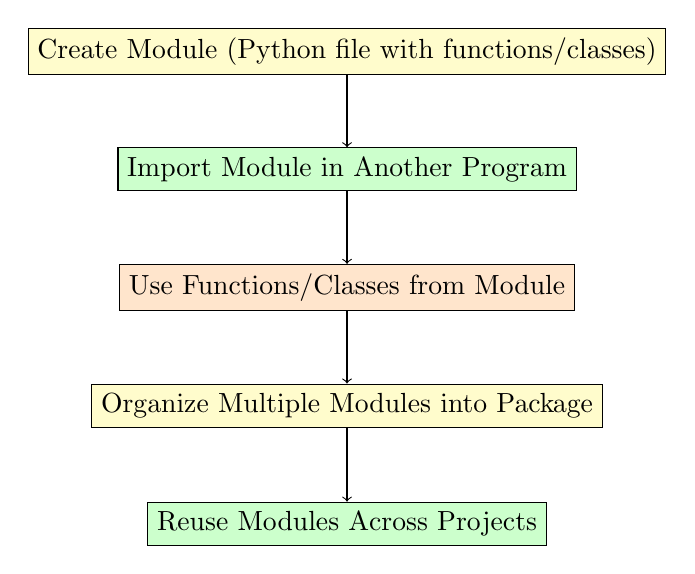
\begin{tikzpicture}[node distance=1.5cm]
\node (module) [draw, rectangle, fill=yellow!20] {Create Module (Python file with functions/classes)};
\node (import) [draw, rectangle, fill=green!20, below of=module] {Import Module in Another Program};
\node (use) [draw, rectangle, fill=orange!20, below of=import] {Use Functions/Classes from Module};
\node (package) [draw, rectangle, fill=yellow!20, below of=use] {Organize Multiple Modules into Package};
\node (reuse) [draw, rectangle, fill=green!20, below of=package] {Reuse Modules Across Projects};
\draw[->] (module) -- (import);
\draw[->] (import) -- (use);
\draw[->] (use) -- (package);
\draw[->] (package) -- (reuse);
\end{tikzpicture}
\end{center}

\section{Key Concepts}

\begin{itemize}
    \item \textbf{Modules}: Python files containing reusable code  
    \item \textbf{Packages}: Directories containing multiple modules  
    \item \textbf{Import} allows using functions and classes from other files  
    \item Encourages \textbf{code organization and reusability}  
    \item Built-in modules save time for \textbf{common tasks}  
\end{itemize}

\section{End-of-Chapter Exercises}

\begin{exercise}{Very Short Questions}
\begin{enumerate}
    \item What is a Python module?  
    \item What is a Python package?  
    \item Name two built-in Python modules.  
\end{enumerate}
\end{exercise}

\begin{exercise}{Short Answer Questions}
\begin{enumerate}
    \item Write a module with a function to calculate the square of a number and import it in another file.  
    \item Explain how packages help in large projects.  
    \item How do you import a specific function from a module?  
\end{enumerate}
\end{exercise}

\begin{exercise}{Activity-Based Questions}
\begin{enumerate}
    \item Create a module with string functions: count vowels, reverse string, and capitalize first letters.  
    \item Build a package \texttt{my\_tools} with two modules: \texttt{math\_utils} and \texttt{string\_utils}. Import and use functions in a main program.  
    \item Explore Python’s \texttt{os} module to list all files in a folder and print them.  
\end{enumerate}
\end{exercise}

\section{Teacher Notes}

\marginnote{
\textbf{Learning Objectives:}  
\begin{itemize}
    \item Students can create and use Python modules  
    \item Students understand the structure of packages  
    \item Students can import and reuse code efficiently  
\end{itemize}

\textbf{Teaching Tips:}  
\begin{itemize}
    \item Start with simple modules containing 1–2 functions  
    \item Show how importing reduces repeated code  
    \item Introduce packages gradually for larger projects  
\end{itemize}

\textbf{Assessment:}  
\begin{itemize}
    \item Observe correct module creation and imports  
    \item Check ability to organize code into packages  
\end{itemize}
}